\newpage
\subsection{Calibration}

An ideal MR scanner should exhibit perfect homogeneity in the static field $B_0$, RF transmit field $B_1^+$, and perfect linearity in the gradient fields. Moreover, RF pulses should be perfectly matched to the Larmor frequency of the sample. In practice, no scanner can achieve all these characteristics perfectly. Calibration serves to minimize these discrepancies to promote signal quality.

This module will guide you through calibrating the tabletop scanner in three stages: finding the Larmor frequency of a sample, tuning the RF pulse amplitude to achieve a $90^{\circ}$ tip angle, and shimming (flattening) the $B_0$ field. \textbf{The Larmor frequency calibration is particularly sensitive to environmental changes and should be repeated periodically during each lab session.} Shimming and RF tuning need only be completed once as an exercise for this module.

\textbf{Use a water-only phantom for this module.}

\subsubsection{Finding the Center Frequency} \label{sec:center}

\noindent{}\textbf{Note: this frequency calibration is extremely sensitive to temperature. It is recommended to re-calibrate the center frequency every 10-20 minutes or before any important scan.}
\vspace{3mm}

The \emph{center frequency} describes the carrier frequency for RF excitation pulses as well as the demodulation frequency for signal reception. In both cases we want the center frequency calibrated to the Larmor frequency of the target nuclei at the magnet \emph{isocenter} (point where all gradients are zero). If the center frequency is poorly calibrated, then excitation is said to be off-resonance and the basic tip angle behavior $\theta = \gamma B_1 \tau$ does not hold.
% Spins \emph{may} still become excited (to a lesser degree) but the excited profile will not be as straight-forward.

For $^1 H$ imaging with this 0.26T scanner, the nominal Larmor frequency is: 

$$ f = \frac{\gamma}{2\pi} B_0 = 42.58\,\text{MHz/T} \times 0.26\,\text{T} = 11.1\,\text{MHz} $$

The current center frequency of the tabletop scanner is available in the \textbf{Parameters} menu under \emph{General}, labelled ``RF Frequency [MHz]''. Make a note of this current value to track how it changes over the course of calibration. This is a good practice whenever you are re-calibrating the center frequency.

Relax 2.0 provides two methods for calibrating the center frequency: a coarse search when the error is large, and fine-tuning when the error is small. First let's try the fine-tuning method, which aims to center the frequency spectrum of the received signal.

 \begin{figure}[h]
    \centering
    \vspace{-5mm}
    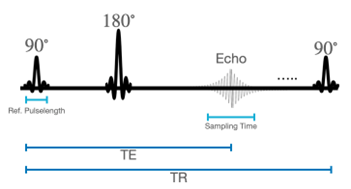
\includegraphics[width=0.7\textwidth]{spin-echo}
    \captionsetup{width=.9\textwidth}
    \caption{\label{fig:calib-spin-echo} Sequence diagram for a non-selective spin echo sequence used to calibrate the center frequency. No gradients are active. The echo envelope is determined by T2* decay.}
    %\vspace{-5mm}
\end{figure}

\begin{enumerate}
    \item In the main menu, click \textbf{Spectroscopy} and select the \textbf{Spin Echo} sequence from the drop-down menu. This sequence is depicted in Figure \ref{fig:calib-spin-echo}.
    \item \label{step:params} Open the \textbf{Parameters} menu. Set the following parameters: under \emph{General} set TE to 10 ms, TR to 2000 ms, Sampling Time to 6 ms; under \emph{Config \& Misc} set 90 Ref. RF Pulse Length to 100 $\mu$s, RF Attenuation to -10 dB.
    \item \label{step:acquire} Return to the main menu. Click \textbf{Acquire}. Wait for the spin echo sequence to run.
    \item \label{step:process} Click \textbf{Data Process}. Observe the two resulting figures plotting the received signal in time and frequency domains. Note these plots show the received signal \emph{after demodulation} by the current center frequency. Try adjusting the frequency range in the Plotvalues window to zoom in on the peak. This can help visualize any bias in the center frequency.
    \item \label{step:recenter} Calibrate the center frequency by navigating to the \textbf{Parameters} menu and clicking \textbf{Recenter} under the center frequency field. % This will update the center frequency according to the bias of the resonant peak in the frequency spectrum. TODO check code to see if this is actually how it works
    \item Repeat steps \ref{step:acquire} to \ref{step:recenter}. A well-calibrated center frequency should result in a sharp peak at 0 in the (demodulated) frequency spectrum. Also, there should be minimal exchange between the real \& imaginary parts in the time domain plot. Thus you can use these two plots to visually assess the quality of your calibration. If the results are poor, try repeating this step once more. If the results are still poor then do the coarse search method below for a better initial value.
\end{enumerate}

If the fine-tuning method was unsuccessful, try the coarse search method. The approach here is to iterate over different center frequencies and record the peak signal, which should be highest at the Larmor frequency.

\begin{enumerate}
    \item Use the same timing parameters as for the fine-tuning method (step \ref{step:params} above).
    \item Navigate to the main menu. Click \textbf{Tools} and locate the \emph{AutoCenter} tool.
    \item Find the note on the magnet box with an approximate center frequency for this particular magnet (e.g. 11.25 MHz).
    \item Set the \emph{AutoCenter} start \& end frequencies to span a 0.1 MHz range centered on the value you found noted on the magnet box. Set the iteration step size to 5000 Hz.
    \item Click \textbf{Go}. The AutoCenter tool will take a few minutes to run. 
    \item When the tool finishes, navigate to the \textbf{Parameters} menu and update the center frequency by clicking the \textbf{Set to Tool Ref} button under the RF Frequency field.
    \item Try the fine-tuning method again.
\end{enumerate}

\noindent{}\color{red}When you are satisfied with the calibration result, capture a screenshot of the two figure windows alongside the Plotvalues window reporting center frequency, FWHM, SNR, and B0 inhomogeneity. These are useful metrics for understanding signal quality. It is a good practice to pay attention to how these values change over the course of calibration.
\color{black}

\subsubsection{RF Attenuation}

The RF Attenuation calibration adjusts the RF Pulse Amplitude to achieve a $90^{\circ}$ tip angle.

\begin{enumerate}
  \item Navigate to the main menu. Click \textbf{Spectroscopy} and select \textbf{Spin Echo} from the drop-down menu. Use the same parameters as in \ref{sec:center}.
  \item Navigate to the main menu. Click \textbf{Tools} and locate the \emph{TrAdj} (Transmit Adjust) tool. Set the attenuation range to [-20, -1] dB with 20 steps. 
  \item Click \textbf{Go}. This will take a minute to run.
  \item When the tool is finished, you will see a plot of signal vs RF attenuation. A $90^{\circ}$ tip angle is achieved where the signal is maximal. This value is reported in the Tools window in the Ref Attenuation field.
  \item Set RF attenuation to this value in the \textbf{Parameter} menu. This can be done automatically by clicking \textbf{Set to Tool Ref} under the RF Attenuation field. 
  \item Run the Spectroscopy Spin Echo sequence again (\textbf{Acquire}) and visualize the result (\textbf{Data Process}). Your signal should be improved. Re-center the center frequency as it may have shifted.  
\end{enumerate}

\noindent{}\color{red}Screenshot the RF attenuation plot. Report the value you find for RF Attenuation to achieve $90^{\circ}$ tip angle.
\vspace{5mm}

\noindent{}\color{red}Capture a screenshot of your improved spin-echo spectrum. What do you notice is different than before? You can also reference statistics from the Plotvalues window for comparison.
\color{black}

\subsubsection{Shimming} 

\noindent{}Shimming is used to improve homogeneity of the main field $B_0$. We do this by adding small, constant currents (DC) to each of the gradient coils. The Z2 channel is exclusively used for shimming whereas the other three gradients X/Y/Z also serve to enable spatial localization, as we will see in upcoming modules.

\vspace{5mm}

\noindent{} Maximizing the homogeneity of the magnetic field corresponds to narrowing the frequency spectrum of a pure sample. Hence we can evaluate the quality of shimming by measuring the height and width of a pure sample's resonant peak in the frequency spectrum. The spectral area should be constant (proportional to number of protons magnetized), so improving the field homogeneity should result in a higher peak with smaller FWHM (full width at half maximum).

\vspace{5mm}

\noindent{} Shimming can be quite time-consuming, so we have already shimmed these systems for you. Instead of having you repeat this entire process, we will have you re-do the shim calibration for just one of the gradients to understand the process and observe the effect on signal quality.

\begin{enumerate}
  \item Find the current shim settings in \textbf{Parameters} under \emph{Config \& Misc}.
  \noindent{}\color{red} Record the current shim settings for Shim X, Shim Y, Shim Z, and Shim Z2. 
  \color{black}
  \item Shift the Shim X value by 50 mA.
  \item \label{step:spin-echo} Run a spectroscopy spin echo (same as you did previously to find the center frequency). You should find that the change to Shim X worsens (increases) the B0 inhomogeneity.
  
  \noindent{}\color{red} Capture a screenshot of the resulting plots.
  \color{black}
  \item Click \textbf{Tools} and locate the \emph{Shim} tool section. This tool serves to test different shim values for a selected gradient. 
  \item Select the X gradient in the tool menu. Set the range of values to span 100 mA centered on the original value of Shim X you recorded above. Set the number of steps to 20.
  \item Click \textbf{Go}. This will take a minute.
  \item After the tool runs you will see a plot of signal versus shim value.
  
    \noindent{}\color{red}
  Capture a screenshot of this plot.
  \color{black}
  \item Repeat the above process once more with a refined range of 10 values spanning 10 mA centered on the optimal value you found from the first run.
  \item The shim value for which peak signal is achieved will be reported in the tool window. Update the Shim X value in the \textbf{Parameters} menu accordingly.
  
  \color{black}
     \noindent{}\color{red}
  Report the optimal Shim X value you found.
  \color{black}
  \item Repeat step \ref{step:spin-echo}.
\end{enumerate}

\noindent{}\color{red} Comment on the difference in signal quality (e.g. B0 inhomogeneity) between the three shim settings: pre-calibration, shifted by 50 mA, and post-calibration.
\color{black}

Throughout this lab you will want to keep B0 inhomogeneity below 50 ppm to ensure reasonably accurate measurements. You can always check this value by acquiring a spectroscopy spin echo and inspecting the Plotvalues window.
\vspace{5mm}

\noindent{} This concludes the calibration module. You have a working scanner! Now is a good time to clean up the desktop as you have likely accrued many windows. You can clear all program windows at once by simply terminating the Relax 2.0 Python program.




